\documentclass{article}
\usepackage{amsmath, sfmath, multicol, tkz-euclide, array, enumerate, tcolorbox, tabularray}
\renewcommand{\familydefault}{\sfdefault}
\setlength{\parindent}{0cm}
\pagestyle{empty}
\usepackage[left=1in, top=0.5in, right=1in, bottom=0.5in]{geometry}
\tikzset{>=stealth}
\tcbset{colback=white}

\newcounter{example}[section]
\newenvironment{example}[1][]{\refstepcounter{example}\par\medskip
   {\color{red}\textbf{Example~\theexample. #1}}}{\medskip}

\begin{document}

\section*{Angle Pairs}

\begin{tcolorbox}[colframe=orange!70!white, coltitle=black, title=\textbf{Today I Can}]
\begin{enumerate}
    \item Identify special angle pairs and use their relationships to find angle measures.
\end{enumerate}
\end{tcolorbox}

\begin{tcolorbox}[colframe=black!20!white, opacitybacktitle=0.1, coltitle=black, title=\textbf{Adjacent Angles}]
\textbf{Adjacent angles} are two angles that \newline 

\begin{minipage}{0.5\textwidth}
\begin{itemize}
    \item Share a common side
    \item Share a common vertex
    \item Have no common interior points
\end{itemize}
\end{minipage}
\begin{minipage}{0.3\textwidth}
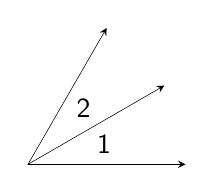
\begin{tikzpicture}
\tkzDefPoints{0/0/A, 2/0/B}
\tkzDefShiftPoint[A](30:2){C}
\tkzDefShiftPoint[A](60:2){D}
\tkzDrawSegment[->](A,B)
\tkzDrawSegment[->](A,C)
\tkzDrawSegment[->](A,D)
\tkzLabelAngle(B,A,C){$1$}
\tkzLabelAngle(C,A,D){$2$}
\end{tikzpicture}
\end{minipage}
\end{tcolorbox}

\begin{tcolorbox}[colframe=black!20!white, opacitybacktitle=0.1, coltitle=black, title=\textbf{Vertical Angles}]
\textbf{Vertical angles} are two angles that are formed by intersecting lines. \newline 

\begin{minipage}{0.3\textwidth}
    \begin{itemize}
        \item $\angle 1$ and $\angle 2$
        \item $\angle 3$ and $\angle 4$
    \end{itemize}
\end{minipage}
\begin{minipage}{0.3\textwidth}
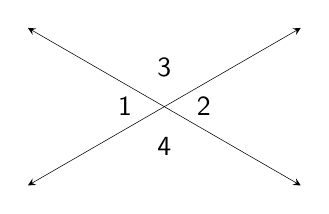
\begin{tikzpicture}
\tkzDefPoints{0/0/A}
\tkzDefShiftPoint[A](30:2){B}
\tkzDefShiftPoint[A](-30:2){C}
\tkzDefShiftPoint[A](150:2){D}
\tkzDefShiftPoint[A](210:2){E}
\tkzDrawSegments[<->](B,E C,D)
\tkzLabelAngle[pos=0.5](D,A,E){1}
\tkzLabelAngle[pos=0.5](C,A,B){2}
\tkzLabelAngle[pos=0.5](B,A,D){3}
\tkzLabelAngle[pos=0.5](D,A,B){4}
\end{tikzpicture}
\end{minipage}
\end{tcolorbox}

\begin{tcolorbox}[colframe=black!20!white, opacitybacktitle=0.1, coltitle=black, title=\textbf{Complementary Angles}]
Two (or more) angles that add to $90^\circ$
\newline 
\begin{minipage}{0.4\textwidth}
    \begin{itemize}
        \item $m\angle 1 + m\angle 2 = 90^\circ$
    \end{itemize}
\end{minipage}
\begin{minipage}{0.4\textwidth}
\begin{tikzpicture}
\tkzDefPoints{0/0/A, 2/0/B, 0/2/C}
\tkzDefShiftPoint[A](30:2){D}
\tkzDrawSegments[->](A,B A,C A,D)
\tkzMarkRightAngle(B,A,C)
\tkzLabelAngle[pos=0.75](B,A,D){1}
\tkzLabelAngle[pos=0.65](D,A,C){2}
\end{tikzpicture}
\end{minipage}
\end{tcolorbox}

\begin{tcolorbox}[colframe=black!20!white, opacitybacktitle=0.1, coltitle=black, title=\textbf{Supplementary Angles}]
Two (or more) angles that add to $180^\circ$
\newline 
\begin{minipage}{0.4\textwidth}
    \begin{itemize}
        \item $m\angle 1 + m\angle 2 = 180^\circ$
    \end{itemize}
\end{minipage}
\begin{minipage}{0.4\textwidth}
\begin{tikzpicture}
\tkzDefPoints{0/0/A, 2/0/B, -2/0/C}
\tkzDefShiftPoint[A](50:2){D}
\tkzDrawSegments[->](A,B A,C A,D)
\tkzLabelAngle[pos=0.5](B,A,D){1}
\tkzLabelAngle[pos=0.25](D,A,C){2}
\end{tikzpicture}
\end{minipage}
\end{tcolorbox}

\begin{example}
Use the diagram to determine if each statement is true. \bigskip 

\begin{minipage}{0.5\textwidth}
\begin{enumerate}[(a)]  \setlength{\itemsep}{1.25cm}
    \item $\angle BFD$ and $\angle CFD$ are adjacent angles.
    \item $\angle AFB$ and $\angle EFD$ are vertical angles.
    \item $\angle AFE$ and $\angle BFC$ are complementary.
\end{enumerate}
\end{minipage}
\hspace{-0.25in}
\begin{minipage}{0.5\textwidth}
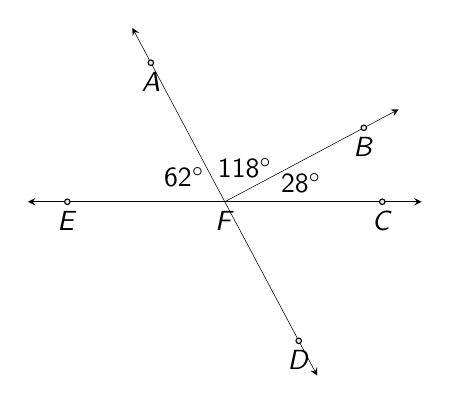
\begin{tikzpicture}
    \tkzDefPoints{0/0/F, 2/0/C}
    \tkzDefShiftPoint[F](28:2){B}
    \tkzDefShiftPoint[F](118:2){A}
    \tkzDefShiftPoint[F](180:2){E}
    \tkzDefShiftPoint[F](-62:2){D}
    \tkzDrawSegments[add = 0 and 0.25, ->, >=stealth](F,A F,B F,C F,D F,E)
    \tkzLabelPoints(A,B,C,D,E,F)
    \tkzDrawPoints(A,B,C,D,E)
    \tkzLabelAngle(C,F,B){$28^\circ$}
    \tkzLabelAngle[pos=0.6](A,F,E){$62^\circ$}
    \tkzLabelAngle[pos=-0.5](E,F,D){$118^\circ$}
\end{tikzpicture}
\end{minipage}
\end{example}

\newpage 

\subsection*{Diagram Assumptions}

It is \textbf{NOT} safe to assume the following from a diagram:
\begin{itemize}
    \item Angles or segments that look congruent actually are.
    \item An angle that looks like a right angle is a right angle.
    \item Angles are complementary.
\end{itemize}

\begin{example}
Can you make each conclusion from the information in the diagram? Explain.
\newline

\begin{minipage}{0.5\textwidth}
\begin{enumerate}[(a)]  \setlength{\itemsep}{1cm}
    \item $\overline{TW} \cong \overline{WV}$
    \item $\overline{PW} \cong \overline{WQ}$
    \item $\angle TWQ$ is a right angle
    \item $\overline{TV}$ bisects $\overline{PQ}$
\end{enumerate}
\end{minipage}
\begin{minipage}{0.5\textwidth}
\begin{tikzpicture}
    \tkzDefPoints{0/0/W, -2/0/P, 2/0/Q, 0/2/T, 0/-2/V}
    \tkzDrawSegments(P,Q T,V)
    \tkzDrawPoints(P,Q,T,V)
    \tkzLabelPoints[below](P,Q)
    \tkzLabelPoints[below right](W)
    \tkzLabelPoints[right](T,V)
    \tkzMarkSegments[mark=|](T,W W,V)
\end{tikzpicture}
\end{minipage}
\end{example}

\begin{tcolorbox}[colframe=black!20!white, opacitybacktitle=0.1, coltitle=black, title=\textbf{Linear Pair}]
Two adjacent angles whose non-common side forms a line. \newline 

\begin{minipage}{0.6\textwidth}
    \begin{itemize}
        \item  $\angle ABD$ and $\angle CBD$ form a linear pair.
    \end{itemize}
\end{minipage}
\begin{minipage}{0.3\textwidth}
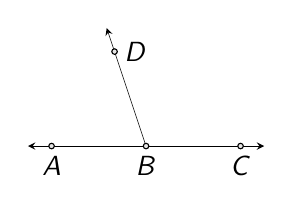
\begin{tikzpicture}[scale=0.8]
    \tkzDefPoints{0/0/A, 1.5/0/B, 3/0/C, 1/1.5/D}
    \tkzDrawSegments[add = 0 and 0.25, ->, >=stealth](B,A B,C B,D)
    \tkzDrawPoints(A,B,C,D)
    \tkzLabelPoints[below](A,B,C)
    \tkzLabelPoints[right](D)
\end{tikzpicture}
\end{minipage}
\end{tcolorbox}

\begin{example}
Find the $m\angle KPL$ and $m\angle JPL$ in the diagram.
\newline\\

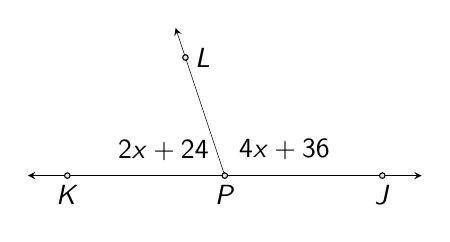
\begin{tikzpicture}
    \tkzDefPoints{0/0/K, 2/0/P, 4/0/J, 1.5/1.5/L}
    \tkzDrawSegments[add = 0 and 0.25, ->, >=stealth](P,K P,J P,L)
    \tkzDrawPoints(K,P,J,L)
    \tkzLabelPoints[below](K,P,J)
    \tkzLabelPoints[right](L)
    \tkzLabelAngle[pos=0.1, above left](L,P,K){$2x+24$}
    \tkzLabelAngle[pos=0.1, above right](J,P,L){$4x+36$}
\end{tikzpicture}
\end{example}

\vfill 

\begin{example}
$\angle ADB$ and $\angle BDC$ form a linear pair. $\angle ADB = 3x+14$ and $\angle BDC = 5x-2$. What are $m\angle ADB$ and $m\angle BDC$?
\end{example}

\vfill 
\newpage 

\begin{tcolorbox}[colframe=black!20!white, opacitybacktitle=0.1, coltitle=black, title=\textbf{Angle Bisector}]
A line, ray, or segment that divides an angle into 2 congruent angles. \newline 

\begin{minipage}{0.6\textwidth}
    \begin{itemize}
        \item $\overrightarrow{AY}$ bisects $\angle XAZ$, so $\angle XAY \cong \angle ZAY$
    \end{itemize}
\end{minipage}
\begin{minipage}{0.3\textwidth}
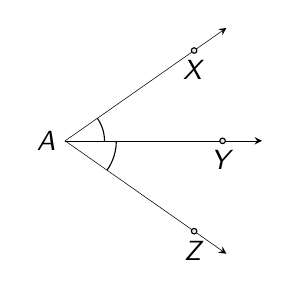
\begin{tikzpicture}
    \tkzDefPoints{0/0/A, 2/0/Y}
    \tkzDefShiftPoint[A](35:2){X}
    \tkzDefShiftPoint[A](-35:2){Z}
    \tkzDrawSegments[->, >=stealth, add = 0 and 0.25](A,X A,Z A,Y)
    \tkzDrawPoints(X,Y,Z)
    \tkzLabelPoints[below](X,Y,Z)
    \tkzLabelPoints[left](A)
    \tkzMarkAngle[size=0.5](Y,A,X)
    \tkzMarkAngle[size=0.65](Z,A,Y)
\end{tikzpicture}
\end{minipage}
\end{tcolorbox}

\begin{example}
$\overrightarrow{AC}$ bisects $\angle DAB$. What is $m\angle DAB$?
\newline\\

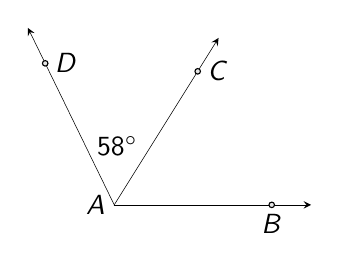
\begin{tikzpicture}
\tkzDefPoints{0/0/A, 2/0/B}
\tkzDefShiftPoint[A](58:2){C}
\tkzDefShiftPoint[A](116:2){D}
\tkzDrawSegments[add = 0 and 0.25, ->, >=stealth](A,B A,C A,D)
\tkzDrawPoints(B,C,D)
\tkzLabelPoints[right](D,C)
\tkzLabelPoints[left](A)
\tkzLabelPoints[below](B)
\tkzLabelAngle[pos=0.75](C,A,D){$58^\circ$}
\end{tikzpicture}
\end{example}

\vspace{0.25in} 

\begin{example}
$\overrightarrow{KM}$ bisects $\angle JKL$. If $m\angle JKL = 72^\circ$, what is $m\angle JKM$?
\end{example}

\vfill 

\begin{example}
In the diagram, $RQ$ bisects $angle PRS$, Find the value of $x$.
\newline\\

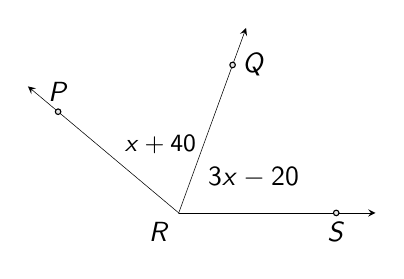
\begin{tikzpicture}
    \tkzDefPoints{0/0/R, 2/0/S}
    \tkzDefShiftPoint[R](70:2){Q}
    \tkzDefShiftPoint[R](140:2){P}
    \tkzDrawSegments[add = 0 and 0.25, ->, >=stealth](R,S R,P R,Q)
    \tkzDrawPoints(P,Q,S)
    \tkzLabelPoints[above](P)
    \tkzLabelPoints[right](Q)
    \tkzLabelPoints[below](S)
    \tkzLabelPoints[below left](R)
    \tkzLabelAngle[pos=0.9](Q,R,P){\small $x+40$}
    \node at (0.25,0.2) [anchor = south west] {$3x-20$};
\end{tikzpicture}
\end{example}

\vfill 

\end{document}
